\chapter{Exchange Arguments and Greedy Algorithms}
\setcounter{section}{-1}   % sections start at 7.0 (see main.tex comment)
\label{ch:exc}

\begin{objectives}
\item Recognize when a selection or ordering problem admits an exchange certificate,
  and which structure buys it.
\item Build the exchange: name the partner, count the swap's delta, pick the
  certificate.
\item Match rung to structure: exact (matroid), $1-1/e$ (submodular), $\ln$
  (cover), $3+\varepsilon$ (metric), complete (symmetry).
\item Dissect a paper's greedy: what is committed, what is swapped, what the factor
  is against.
\end{objectives}

A greedy algorithm commits irrevocably: it keeps one plan out of thousands, merges two
chunks, adds one edge to a forest, fixes the order in which an exact search tries
values. The exchange argument is the certificate that makes such myopia safe: it shows
that any solution avoiding the greedy's choice can be \emph{rearranged} --- one
element, edge, or branch swapped for another --- into a solution that honors it, at a
loss that is either zero (the greedy is exactly optimal, or the pruning loses nothing)
or bounded and countable (the greedy keeps a $1-1/e$ or $\ln$ fraction of the optimum).
For a systems paper this converts ``greedy worked well in our experiments'' into a
theorem, and the theory section often shrinks to checking a hypothesis: independence,
diminishing returns, a covering constraint, metric distances, or symmetry. In the
SIGMOD'26 corpus, 17 tagged papers use the tool; in the tag co-occurrences it pairs
with hardness 10 times and with an approximation-ratio property 9 times --- the
signature of ``NP-hard, but structured'' --- and with correctness 7 times, its
exact-rung twin.

This chapter builds the ladder first: the exchange principle, greedy-stays-ahead, the
matroid rung, and the three factor rungs (submodular, set-cover, metric swaps), each
with its swap accounting. Sections~\ref{sec:exc-053}--\ref{sec:exc-009} then dissect
four corpus exemplars at full anatomy; Section~\ref{sec:exc-advanced} adds two
sketched exemplars and further reading.

\section{The tool: exchange arguments and greedy with certificates}
\label{sec:exc-tool}

The problem class is uniform across applications: a solution must be built or selected
incrementally, under constraints, and each increment is irrevocable. The optimizer
keeps a small set of plans, the sampler picks anchors one at a time under a budget,
the temporal index decides edge by edge what a forest remembers, the exact search
commits to a branching order. A greedy algorithm makes each choice by a myopic rule
--- take the plan covering the most workload, the anchor with the best marginal
fidelity, the heaviest edge that keeps a forest, the first value in a fixed order.
What the exchange argument adds is the after-the-fact certificate: a proof that any
solution avoiding the greedy's commitment can be rearranged into one that honors it.
The organizing question of this chapter is which \emph{structure} buys which
\emph{certificate}: independence (matroids) buys exactness, diminishing returns
(submodularity) buys $1-1/e$, covering buys $\ln$, metrics buy $3+\varepsilon$, and
symmetry buys prune-safety --- completeness with no factor at all.

\begin{remarkbox}[Notation]
$U$ is a ground set, $\mathcal{F}\subseteq 2^U$ a feasible family, $w$ (linear
objectives) or $f$ (set functions) the objective to maximize unless said otherwise.
$S_i$ is greedy's set after $i$ picks; $\Delta(u \mid S) = f(S\cup\{u\}) - f(S)$ is
the \emph{marginal gain}; $y$ always names the \emph{exchange partner} --- the
element of the optimal solution that a swap gives up; $O$ denotes an optimal solution
and $\operatorname{OPT}$ its value. $H(n) = \sum_{i=1}^{n} 1/i$ is the harmonic
number. Maximization rungs quote factors $\le 1$ (as $1-1/e$); minimization rungs
quote factors $\ge 1$ (as $H(n)$, $3+\varepsilon$).
\end{remarkbox}

\subsection{The ladder: from exact exchange to logarithmic coverage}
\label{sec:exc-ladder}

The bottom rung is not a theorem about any one problem but the shape of every proof to
come: an optimal solution can be rearranged, one swap at a time, to agree with the
greedy's choices.

\begin{proposition}[Exchange principle]\label{prop:exc-principle}
Let $\mathcal{F}\subseteq 2^U$ be a feasible family and $w\colon\mathcal{F}\to\mathbb{R}$
an objective to maximize. Let $g$ be greedy's first choice, and suppose that for every
feasible $S$ with $g\notin S$ there is an exchange partner $y\in S$ such that
$S' = (S\setminus\{y\})\cup\{g\}$ is feasible with $w(S')\ge w(S)$, and that the same
condition holds recursively on the residual instance with ground set $U\setminus\{g\}$.
Then greedy returns an optimal solution. \eop
\end{proposition}

\begin{proof}
Induction on $|U|$. Let $O$ be optimal. If $g\in O$, then $O\setminus\{g\}$ is optimal
for the residual instance --- any better residual solution would combine with $g$ to
beat $O$ --- and greedy on the residual returns it by hypothesis. If $g\notin O$, the
swap produces an optimal $O' = (O\setminus\{y\})\cup\{g\}$ containing $g$, which
reduces to the first case.
\end{proof}

\begin{figure}[t]
\centering
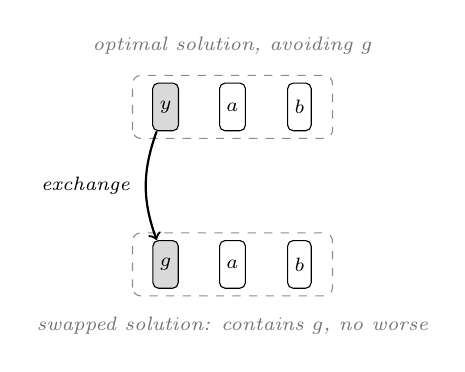
\begin{tikzpicture}[
  every node/.style={font=\scriptsize},
  tok/.style={draw, rounded corners=2pt, inner sep=2.5pt, minimum height=4ex}]
% top row: an optimal solution avoiding g
\node[tok, fill=black!15] (y) at (0,0) {$y$};
\node[tok] (a) at (0.85,0) {$a$};
\node[tok] (b) at (1.7,0) {$b$};
\draw[dashed, rounded corners=3pt, black!45] (-0.42,-0.4) rectangle (2.12,0.4);
\node[text=black!55] at (0.85,0.78) {\itshape optimal solution, avoiding $g$};
% bottom row: the swapped solution
\node[tok, fill=black!15] (g) at (0,-2.0) {$g$};
\node[tok] (a2) at (0.85,-2.0) {$a$};
\node[tok] (b2) at (1.7,-2.0) {$b$};
\draw[dashed, rounded corners=3pt, black!45] (-0.42,-2.4) rectangle (2.12,-1.6);
\node[text=black!55] at (0.85,-2.78) {\itshape swapped solution: contains $g$, no worse};
\draw[->, thick] (y) to[bend right=20]
  node[midway, left=2pt] {\scriptsize\itshape exchange} (g);
\end{tikzpicture}
\caption{The exchange step. Greedy commits to $g$; an optimal solution avoiding $g$
is rearranged into a no-worse solution containing it, one swap at a time. Exact rungs
pay nothing per swap; factor rungs lose a bounded, countable amount that compounds
into the factor.}
\label{fig:exc-swap}
\end{figure}

The next rung makes the rearrangement concrete and shows the craft in miniature: order
the choices well, and the partner swap loses nothing.

\begin{theorem}[Greedy stays ahead]\label{thm:exc-staysahead}
Among all sets of pairwise non-overlapping intervals, the greedy that repeatedly
chooses the compatible interval of \emph{earliest finish time} returns one of maximum
cardinality. \eop
\end{theorem}

\begin{proof}
Write $g_1,g_2,\dots$ for greedy's picks, $o_1,o_2,\dots$ for any optimal solution's,
and $f(\cdot)$ for finish times. By induction, $f(g_i)\le f(o_i)$ for every $i$: it
holds for $i=1$ because greedy takes the earliest-finishing interval of all; and if it
holds for $i$, then $o_{i+1}$ starts at or after $f(o_i)\ge f(g_i)$, so $o_{i+1}$ is
compatible with $g_1,\dots,g_i$ and greedy's $(i{+}1)$-st pick finishes no later than
$o_{i+1}$. Greedy is never behind, so it cannot stop earlier: if the optimum had a
$(k{+}1)$-st interval, it would be compatible with $g_1,\dots,g_k$, and greedy would
have had a choice at step $k{+}1$.
\end{proof}

When the feasibility of each swap is governed by an \emph{independence structure}, the
principle industrializes into an exact algorithm for a whole problem class.

\begin{definition}[Matroid]\label{def:exc-matroid}
A pair $(U,\mathcal{I})$ with $\mathcal{I}\subseteq 2^U$ is a \emph{matroid} if
(i)~$\mathcal{I}$ is hereditary --- $S\in\mathcal{I}$ and $S'\subseteq S$ imply
$S'\in\mathcal{I}$ --- and (ii)~it satisfies the \emph{exchange axiom}: if
$A,B\in\mathcal{I}$ with $|A|<|B|$, then $A\cup\{x\}\in\mathcal{I}$ for some
$x\in B\setminus A$. Members of $\mathcal{I}$ are called \emph{independent} sets.
\end{definition}

\begin{theorem}[Matroid greedy is exact, Edmonds]\label{thm:exc-matroid}
On a matroid, the greedy that scans elements in nonincreasing weight order and keeps
each element that preserves independence returns a maximum-weight independent set ---
for every weight function. Conversely, if greedy is exact for every weight function,
then the family of independent sets satisfies the exchange axiom, so the structure is
a matroid \citep{exchange-greedy-bg1}. \eop
\end{theorem}

\begin{proof}[Proof idea]
The exchange axiom is Proposition~\ref{prop:exc-principle}'s one-for-one swap with
zero loss: if the optimum ``spends'' $y$ where greedy spent $g$ with $w(g)\ge w(y)$,
swap. The full induction is in Section~\ref{sec:exc-appendix}.
\end{proof}

\sidenote{The graphic matroid takes $U$ to be a graph's edges and
$\mathcal{I}$ its forests (acyclic edge sets); maximal independent sets are spanning
forests, and the cycle rule --- an edge that closes a cycle may replace the lightest
edge of that cycle --- is the exchange axiom in the wild. Kruskal's algorithm is the
matroid greedy; the union--find structure that implements it reappears in
Section~\ref{sec:exc-200}.}

Outside matroids exactness dies, but diminishing returns keep a quantitative exchange
alive: greedy's next pick matches the \emph{average} marginal value of the optimum's
remaining elements.

\begin{definition}[Monotone submodular]\label{def:exc-submodular}
$f\colon 2^U\to\mathbb{R}_{\ge 0}$ is \emph{submodular} if
$f(S\cup\{x\}) - f(S) \;\ge\; f(T\cup\{x\}) - f(T)$ whenever $S\subseteq T\subseteq U$
and $x\in U\setminus T$ (diminishing returns), and \emph{monotone} if $S\subseteq T$
implies $f(S)\le f(T)$.
\end{definition}

\begin{theorem}[Submodular greedy, Nemhauser--Wolsey--Fisher]\label{thm:exc-nwf}
Let $f$ be monotone submodular with $f(\emptyset)=0$, and let $A_B$ be the set built
by $B$ greedy steps, each adding the $u\notin A$ that maximizes $\Delta(u\mid A)$.
Then
\[
f(A_B) \;\ge\; \Bigl(1-\frac{1}{e}\Bigr)\max_{|A|\le B} f(A), \eopm
\]
and the factor $1-1/e$ is tight for maximum coverage unless $P=NP$
\citep{exchange-greedy-bg2,exchange-greedy-bg5}.
\end{theorem}

\begin{proof}[Proof idea]
Each greedy pick captures at least a $1/B$ fraction of the remaining optimality gap,
so the gap contracts by $(1-1/B)$ per step; unrolling $B$ steps gives
$(1-1/B)^{B}\le e^{-1}$ (Section~\ref{sec:exc-appendix}).
\end{proof}

When the objective is a covering constraint in disguise --- cover the universe at
minimum total weight --- the same averaging against the optimum yields the harmonic
factor:

\begin{theorem}[Set-cover greedy, Chv\'atal]\label{thm:exc-cover}
Given a universe of $n$ elements and a family of sets with nonnegative weights, the
greedy that repeatedly buys the set maximizing newly-covered elements per unit weight
returns a cover of total weight at most $H(n)\cdot\operatorname{OPT} \le
(1+\ln n)\operatorname{OPT}$, where $H(n)=\sum_{i=1}^{n}1/i$; the bound sharpens to
$H(d)$ when every set has at most $d$ elements \citep{exchange-greedy-bg3}. \eop
\end{theorem}

\begin{proof}[Proof idea]
While $r$ elements remain uncovered, the sets of an optimal cover jointly cover them
at total weight $\operatorname{OPT}$, so one of them covers at rate at least
$r/\operatorname{OPT}$ per unit weight --- and greedy picks at least that well.
Charging each element the price at which it was covered and summing the harmonic
series gives $H(n)$ (Section~\ref{sec:exc-appendix}).
\end{proof}

The last rung replaces ``take the best now'' with ``swap if it helps'': local search
over exchanges, certified by the metric.

\begin{theorem}[Swap local search for $k$-median, Arya et al.]\label{thm:exc-kmedian}
In metric $k$-median, the local search that repeatedly swaps one center for a
non-center whenever it lowers the total assignment cost terminates at a solution of
cost at most $(3+\varepsilon)\operatorname{OPT}$; allowing multi-swaps of up to $p$
centers improves the factor to $2+\varepsilon$ \citep{exchange-greedy-bg4}. \eop
\end{theorem}

\begin{proof}[Proof idea]
At a local optimum no single swap gains. Charge each optimal center to a nearby local
center: the swap that trades one for the other reassigns points through two triangle
inequalities, and the (non-improving) swap's cost delta bounds
$\operatorname{OPT}$ by three times the local cost.
\end{proof}

The rungs share one mechanism --- the swap --- and differ only in the accounting:
\emph{rearrangement} (delta $\ge 0$, greedy optimal), \emph{contraction} (delta $\ge$
gap$/B$, compounding to $e^{-1}$), \emph{averaging} (delta $\ge$
residual$/\operatorname{OPT}$, compounding to $H(n)$), \emph{two triangle
inequalities} ($3+\varepsilon$). Two corpus exemplars below use rungs with no factor
at all: the swap certifies that a construction is exact or that pruning is safe.

\subsection{How to build the exchange}
\label{sec:exc-build}

The construction procedure is mechanical once the greedy rule is written down.
\emph{First}, state what one step commits to --- an element enters the solution, an
edge enters a forest, a value order is fixed. \emph{Second}, take any optimal solution
$O$ that avoids the commitment and \emph{name the exchange partner} $y$: the element
of $O$ doing the job $g$ would do --- the optimal cover's set that greedy's set
displaces, the optimal forest's edge on the cycle $g$ closes, the optimal branch that
tries the values in the other order. \emph{Third}, \emph{count the swap's cost delta}
for $O' = (O\setminus\{y\})\cup\{g\}$: feasibility of $O'$ comes from the structure
(the exchange axiom, heredity, the cycle property, automorphism invariance, plain
coverage), and the delta comes from the objective's arithmetic --- a weight
comparison, a diminishing-returns inequality, a price-per-element average, two
triangle inequalities, or identical neighborhoods. \emph{Fourth}, read off the
certificate type from the delta: zero loss with self-similar residuals gives
exactness; a $1/B$ fraction of the gap gives $1-1/e$; a $1/\operatorname{OPT}$
fraction of the residual gives $\ln$; a strictly earlier branch gives completeness.
The audit effort goes into the \emph{hypothesis}, not the algorithm: submodularity by
pairwise marginal tests or a concave-gain decomposition, the exchange axiom by an
independence oracle, metric structure by the triangle inequality, symmetry by
automorphisms. Near-modular or noisy objectives void the certificate --- and an
honest paper then says so (Section~\ref{sec:exc-advanced}).

\begin{reachbox}{When to Reach for Exchange/Greedy Arguments}
Reach whenever a selection, covering, or clustering problem has been proved NP-hard
(or an exact search explodes) but the objective carries \emph{checkable} structure,
and the deliverable is an algorithm whose quality is a theorem, not a benchmark: a
factor-certified or exactness-certified polynomial-time procedure. Then run the
recipe:
\begin{enumerate}
\item \textbf{Name the exchange partner.} Fix the greedy's next commitment $g$ and an
  optimal solution $O$ avoiding it; identify the element, edge, center, or branch $y$
  of $O$ that plays $g$'s role.
\item \textbf{Identify the structure} that licenses the swap: matroid independence
  (exact), monotone submodularity ($1-1/e$), a covering constraint ($\ln$), metric
  distances ($3+\varepsilon$ swaps), a symmetry group (pruning stays complete).
\item \textbf{Count the swap's cost delta.} Zero loss, a $1/B$ fraction of the gap, a
  $1/\operatorname{OPT}$ fraction of the residual, two triangle inequalities, or
  identical neighborhoods --- the count determines the certificate.
\item \textbf{State the certificate of near-optimality:} which factor, against which
  optimum, with which slack ($\ln\delta^{-1}$, $\varepsilon$) --- inherited, not
  re-derived. If no structure checks out, say so and call the greedy a heuristic.
\end{enumerate}
\end{reachbox}

\section{Risk coresets for robust query optimization}
\label{sec:exc-053}

The exemplar is a PODS'26 paper on robust query optimization \citep{sigmod26-053}\pods.
Query optimizers pick execution plans using cardinality estimates, and the estimates
can be badly wrong; a plan that looks cheapest under the estimates may be terrible on
the true cardinalities. Robust query optimization therefore scores each plan by
\emph{risk}: the probability, over the uncertainty about cardinalities, that the
plan's cost exceeds a factor $\tau$ of the best plan for the realized instance. The
paper asks for a small \emph{coreset} of plans that covers a whole workload
distribution --- after seeing the coreset, a query-time inference step should pick,
from a few precomputed plans, one nearly as robust as the best plan in the entire
exponential space. Its main result is a greedy-cover algorithm that samples
$O((\kappa^{*}/\delta^{2})\ln N\ln(\delta^{-1}))$ queries from the workload and
computes, with high probability, a coreset of size $O(\kappa^{*}\ln\delta^{-1})$ ---
within a logarithmic factor of the smallest coreset $\kappa^{*}$ that exists --- from
which inference returns a plan of risk at most twice the optimum plus $4\varepsilon$.

\paragraph{Problem.}
Work over a plan set $\Pi$ with $|\Pi| = N$ and a workload distribution $W$ over a
query space $\mathcal{Q}$. Each query $Q$ carries an \emph{uncertainty profile}
$U_Q$: a distribution over cardinality vectors $s$, against which plan costs
$\operatorname{Cost}(\pi,s)$ (linear in $s$) are judged. The \emph{penalty} of $\pi$
at $s$ is its cost ratio against the best plan for $s$,
$\operatorname{Pnl}(\pi,s) = \operatorname{Cost}(\pi,s)/\operatorname{Cost}^{*}(s)$,
and the $\tau$-\emph{risk} of $\pi$ on $Q$ is
$\operatorname{Risk}(\pi,Q;\tau) = \Pr_{s\sim U_Q}[\operatorname{Pnl}(\pi,s)>\tau]$,
with $\operatorname{Risk}^{*}(Q;\tau)$ the minimum over all plans. A plan set
$F\subseteq\Pi$ \emph{covers} query $Q$ when its best plan is nearly as robust as the
overall best, $\min_{\pi\in F}\operatorname{Risk}(\pi,Q;\tau) \le
\operatorname{Risk}^{*}(Q;\tau)+\varepsilon$; the failure probability $p(\varepsilon,F)$
is the $W$-probability that $F$ does not cover $Q$, and $F$ is an
$(\varepsilon,\tau,\delta|W)$-\emph{coreset for risk} when $p(\varepsilon,F)\le\delta$.
Let $\kappa^{*}$ be the size of the smallest such coreset. The goal: compute a valid
coreset of size $O(\kappa^{*}\cdot\operatorname{polylog})$ from few workload samples.

\paragraph{Guarantee.}

\begin{theorem}[Risk coreset via greedy cover; Theorem~3.5 of the paper, notation
cleaned]\label{thm:exc-053-main}
Let $W$ be a workload distribution, $\Pi$ a plan set with $|\Pi|=N$, parameters
$\varepsilon\in(0,1]$, $\tau\ge 1$, $\delta\in(0,1)$, and $\kappa^{*}$ the size of the
smallest $(\varepsilon,\tau,\delta|W)$-coreset for risk. For any constants
$c_1,c_2>1$ there is an algorithm that samples
$O\bigl((\kappa^{*}/\delta^{2})\ln N\ln(\delta^{-1})\bigr)$ queries from $W$ and
computes, in time
$O\bigl((\kappa^{*}/(\varepsilon^{2}\delta^{2}))\cdot N\ln^{3}N\cdot
\ln(\delta^{-1})\bigr)$, a set $C\subseteq\Pi$ of size $O(\kappa^{*}\ln(\delta^{-1}))$
such that, with high probability, $C$ is a $(c_1\varepsilon,\tau,c_2\delta|W)$-coreset
for risk. \eop
\end{theorem}

\sidenote{A \emph{coreset} is a small surrogate that preserves the quality of the
full object; here the object is the plan space and the quality is workload-wide risk
coverage. $\kappa^{*}$ is instance-dependent --- small when a few plans already cover
the workload --- which is why the guarantee is stated relative to $\kappa^{*}$ and not
to $N$.}

\paragraph{How the greedy cover is applied.}
The algorithm runs in rounds indexed by a guess $k_r$ that doubles every round; in
round $r$ it samples $\mathfrak{n}_r = (c_1 k_r/\delta^{2})\ln N\ln(\delta^{-1})$
queries from $W$, estimates each plan's risk on each sampled query from
$\mathfrak{m}_r = (c_2/\varepsilon^{2})\ln N\ln\mathfrak{n}_r$ profiles drawn from the
query's uncertainty profile, and runs a maximum-coverage greedy with budget
$b_r = c_3 k_r\ln(\delta^{-1})$ plans: repeatedly add the plan covering the most
not-yet-covered sampled queries, terminating when at least a $(1-2\delta)$-fraction is
covered. Two estimation lemmas make the greedy's proxies faithful: Lemma~3.1 of the
paper bounds the empirical failure probability by Hoeffding plus a union bound over
all $\le (b_r+1)N^{b_r}$ plan subsets of size at most $b_r$, giving
$|\widehat{p}_r(\varepsilon',F) - p(\varepsilon',F)|\le\delta/4$ simultaneously with
probability $1-N^{-O(1)}$; Lemma~3.2 of the paper does the same per (plan, query)
pair, Hoeffding over the $\mathfrak{m}_r$ risk indicators plus a union bound over the
$N\mathfrak{n}_r$ pairs. So the greedy cover behaves almost as if it saw true risks.
The exchange rung --- averaging against the optimal coreset --- is the workhorse:

\begin{lemma}[Greedy termination; Lemma~3.4 of the paper]\label{lem:exc-053-term}
Assuming the conditions of Lemmas 3.1 and 3.2 of the paper hold in every round, the
algorithm terminates with $k_r \le 2\kappa^{*}$. \eop
\end{lemma}

\begin{proof}[Proof sketch]
By Lemma~3.1 the optimal coreset $M$, $|M| = \kappa^{*}$, covers at least a
$(1-5\delta/4)$-fraction $\mathfrak{n}'$ of the sampled queries, so among $M$'s plans
some covers at least a $1/\kappa^{*}$ fraction of whatever residual $D_t$ remains;
greedy picks at least that well, so $D_{t+1}\le(1-1/\kappa^{*})D_t \le
e^{-t/\kappa^{*}}\mathfrak{n}'$. After $t \ge c_3\kappa^{*}\ln(\delta^{-1})$ rounds
the coverage reaches $1-2\delta$, the termination condition --- so the round with
$k_r\ge\kappa^{*}$ terminates, and doubling gives $k_r\le 2\kappa^{*}$. (Full proof in
Section~\ref{sec:exc-appendix}.)
\end{proof}

Deployment adds two transfer steps, both exchange-flavored. Lemma~4.2 of the paper
converts \emph{local} risks (against the coreset $F$) into \emph{global} risks:
\[
\operatorname{Risk}(\pi,Q;\tau^{2}) \;\le\;
\operatorname{L-Risk}_{F}(\pi,Q;\tau) \;+\;
\min_{\pi'\in F}\operatorname{Risk}(\pi',Q;\tau),
\]
so minimizing over $\pi\in F$ bounds the global $\tau^{2}$-risk by twice the best
$\tau$-risk in $F$. Lemma~4.6 of the paper is a Markov step: if $C$ is an
$(\alpha,\delta_1\delta_2|W)$-coreset for neighborhood cost, then the neighborhood
error-rate $N_{\alpha,C}(Q)$ --- the $U_Q$-probability that no plan of $C$ is within
factor $\alpha$ of optimal --- satisfies $\Pr_{Q\sim W}[N_{\alpha,C}(Q)>\delta_1]
\le\delta_2$, because $\mathbb{E}[N_{\alpha,C}(Q)]\le\delta_1\delta_2$ and Markov caps
the tail. Together these give the paper's Theorem~4.1: the inference step, which
scores each coreset plan by its empirical local risk on
$\Theta((\ln|F|+\ln\delta^{-1})/\varepsilon^{2})$ sampled profiles, returns with
probability $1-2\delta$ a plan $\hat{\pi}$ with
$\operatorname{Risk}(\hat{\pi},Q;\tau^{2}) \le 2\operatorname{Risk}^{*}(Q;\tau)+4\varepsilon$.

\paragraph{What it buys.}
The optimizer precomputes once a plan set of size $O(\kappa^{*}\ln\delta^{-1})$ ---
logarithmic slack over the best possible --- and every arriving query is answered by
argmin over that set, in $\Theta(|F|(\ln|F|+\ln\delta^{-1})/\varepsilon^{2})$ time,
with a certified worst-case robustness contract. The greedy cover inherits the
set-cover factor; the Hoeffding and Markov layers only make the cover's input
faithful.

\section{Cohesive subgraphs in temporal graphs, exactly}
\label{sec:exc-200}

The exemplar is a SIGMOD'26 paper on temporal graph queries \citep{sigmod26-200}.
Temporal graphs record when each edge was alive, and analysts routinely ask for
\emph{cohesive subgraphs} --- connected components, $k$-cores, connected $k$-cores ---
restricted to an arbitrary time window: ``the community active between $t_s$ and
$t_e$.'' Answering from scratch per window means recomputing a decomposition for
every query, which is wasteful when windows overlap heavily. The paper instead builds
a single index that answers such \emph{historical} cohesive-subgraph queries for any
window and any of the three models: an \emph{affiliated forest} --- essentially a
Kruskal-style decomposition of the temporal edges, maintained by union--find with
inverse-Ackermann amortization --- plus a compact search structure over the resulting
3-dimensional intervals (BTAS). The headline: $O(m\log m)$ construction, $O(m)$ space,
and $O(n+\log^{2}m)$ per query, exactly, with no approximation anywhere.

\paragraph{Problem.}
A temporal graph $G=(V,E)$ gives each edge a lifespan $[t_1,t_2]$; the snapshot
$G[t_s,t_e]$ keeps exactly the edges whose entire lifespan lies inside the window. A
\emph{cohesive subgraph model} (CSM) $P$ maps each graph to a set of subgraphs;
$P$ is \emph{non-overlapping} when any two subgraphs it returns have disjoint vertex
sets, and \emph{monotonic} when passing to a supergraph only grows the returned
subgraphs. Lemma~2.3 of the paper verifies both properties for the three models of
interest --- the connected component, the $k$-core, and the connected $k$-core (the
$k$-core case itself by a mini exchange argument: two overlapping $k$-cores union to
a larger one, contradicting maximality, so the $k$-core is unique). A
\emph{Historical-CSM} query gives a window $[t_s,t_e]$ and asks for
$P(G[t_s,t_e])$. Each edge becomes a \emph{spanning edge} $(u,v,t_1,t_2)$ of an
affiliated graph, and a lemma of the paper (its Lemma~3.4) reduces Historical-CSM
queries for any non-overlapping, monotonic CSM to a unified, CSM-free
\emph{Spanning-CC} query on the affiliated graph: find all vertex sets that induce
connected components of the windowed affiliated graph.

\paragraph{Guarantee.}

\begin{theorem}[AF-BTAS index; Lemmas 3.6, 3.12, and 3.13 of the paper,
compressed]\label{thm:exc-200-index}
Let $G=(V,E)$ be a temporal graph with $n$ vertices and $m$ edges, and $P$ a
non-overlapping, monotonic CSM. The construction $\mathsf{BuildAF}$ produces, for
every window $[x,y]$, a spanning forest $(V,F_{x,y})$ of the affiliated graph such
that a spanning edge $e=(u,v,t_1,t_2)$ belongs to $F_{x,y}$ if and only if
$0\le x\le t_1$ and $t_2\le y\le\tau(e)$, where $\tau(e)$ is the eviction time
recorded for $e$ (Lemma~3.6 of the paper); the construction is amortized near-linear
through union--find (Lemma~3.8 of the paper). The index AF-BTAS built on the triples
$(t_1,t_2,\tau(e))$ takes $O(m\log m)$ time and $O(m)$ space and answers a Spanning-CC
query for any window in $O(n+\log^{2}m)$ time. \eop
\end{theorem}

\paragraph{How the exchange argument is applied.}
The rung is the graphic matroid: spanning forests are the independent sets, and the
cycle rule --- an edge that closes a cycle may replace a lighter edge of that cycle ---
is the exchange axiom. The paper's $\mathsf{AFDecomp}$ sweeps the spanning edges once,
in an order $\omega_1$ by interval start; a union--find structure maintains the
current forest $S$. When the arriving edge $e_i=(u,v,t_1,t_2)$ connects two vertices
already connected, it closes a cycle: the algorithm finds the $\omega_2$-minimal edge
$e_{\min}$ on that cycle (the one whose usefulness ends earliest) and \emph{exchanges}
--- if $\omega_2(e_i)>\omega_2(e_{\min})$ then $S \gets (S\cup\{e_i\})\setminus\{e_{\min}\}$
and the eviction time is recorded as $\tau(e_{\min}) = t_2-1$; otherwise $e_i$ is
discarded. Every swap is Kruskal's rule applied to a different weight order, and
Lemma~3.6 is precisely the invariant the swaps preserve: an edge survives in exactly
those windows $[x,y]$ that contain its lifespan and end before its eviction. Edges
never evicted get $\tau(e)=t_{\max}$. Correctness of the decomposition is proved by
induction along the sweep (the paper's proof of its Lemma~3.10 shows the running
forest equals each $F_{0,y}$ in turn), and monotonicity of the CSM guarantees
supersets of $u$--$v$ windows stay $u$--$v$ windows (Lemma~3.2 of the paper). The
$\alpha(\cdot)$-amortized union--find checks make the whole sweep near-linear, and the
resulting triples $(t_1,t_2,\tau(e))$ are answered by BTAS --- a binary tree whose
nodes carry priority search trees for the 3-sided query $x\le t_s\le y\le t_e\le z$ ---
in $O(\log m)$ recursion rounds of $O(\log m)$ each plus output size.

\sidenote{The exchange here earns no approximation factor because nothing is
approximated: the cycle swap maintains a \emph{maximum} forest for every window
simultaneously, and the certificate is completeness --- the index answers every query
exactly. This is the matroid rung of Section~\ref{sec:exc-ladder} deployed as a data
structure.}

\paragraph{What it buys.}
One $O(m\log m)$ preprocessing step turns any-window cohesive-subgraph queries into
output-sensitive $O(n+\log^{2}m)$ lookups, replacing per-query recomputation. The same
index serves all three CSMs because the construction uses only non-overlap and
monotonicity, and the union--find amortization keeps the certificate cheap to earn.

\section{Representative sampling for large-scale vector data}
\label{sec:exc-031}

The exemplar is a SIGMOD'26 paper on sampling for vector data \citep{sigmod26-031}.
Graph-based nearest-neighbor indexes navigate a dataset greedily --- beam search hops
from anchor to anchor toward the query --- so everything depends on the anchors being
well placed: globally spread, yet locally dense enough that navigation does not stall.
The paper studies \emph{representative sampling} under a budget: choose a subset of
data points that balances a global coverage constraint against local fidelity, where
fidelity is measured through the local intrinsic dimension (LID) of each point's
neighborhood. It proves the exact selection problem NP-hard, then designs a fidelity
objective $F$ built from per-point gains and shows that (lazy-)greedy under the budget
returns $F$ at least $1-1/e$ of optimal. A companion analysis shows the same anchor
densities that $F$ rewards also make greedy and beam navigation progress with high
probability, via $(1-p)^{m}\le e^{-mp}$ bounds.

\paragraph{Problem.}
Given a dataset of $n$ vectors, a sampling ratio $\rho$ (budget $B=\lfloor n\rho\rfloor$)
and a coverage budget $C_{\max}$, Problem~1 of the paper (\emph{Representative
Sampling}) asks for a sample $A$ of at most $B$ anchors maximizing a local-fidelity
objective $F(A) = \sum_{s} g_s\bigl(m_s(A)\bigr)$ subject to a coverage constraint
$\operatorname{Cost}_{\mathrm{cov}}(A) = \frac1n\sum_{x}\min_{a\in A}
\operatorname{dist}(x,a) \le C_{\max}$, where $m_s(A)$ counts the selected anchors in
point $s$'s neighborhood ball $B(s)$ and $g_s$ is $s$'s per-anchor fidelity gain. The
problem is intractable exactly: Theorem~2 of the paper proves Problem~1 NP-hard by a
parsimonious reduction from metric $k$-median --- set $\rho \gets k/n$ so the budget
forces $|A| = k$, and $C_{\max} \gets T/n$ so the coverage constraint \emph{is} the
$k$-median objective --- so a feasible sample of size $k$ within budget is precisely a
$k$-median answer.

\paragraph{Guarantee.}

\begin{theorem}[Lazy-greedy representative sampling; Theorem~3 of the paper]
\label{thm:exc-031-gre}
Let $B$ be the budget and $A_{\mathrm{gre}}$ the size-$B$ output of the (lazy-)greedy
algorithm (Algorithm~2 of the paper). Then
\[
F(A_{\mathrm{gre}}) \;\ge\; \Bigl(1-\frac{1}{e}\Bigr)\max_{|A|\le B} F(A). \eopm
\]
\end{theorem}

\paragraph{How the submodular greedy is applied.}
The exchange structure is monotone submodularity, and it is earned, not assumed. The
per-point gains come from an estimation analysis: Lemma~1 of the paper represents the
LID estimator at $s$ as $D\cdot(\sum_{j\le m}Y_j)^{-1}$ with $Y_j\sim\mathrm{Exp}(1)$
i.i.d.\ (so $Z=\sum_j Y_j\sim\Gamma(m,1)$), and its gamma-sum moment identities give
closed forms --- mean $D\,m/(m-1)$, variance $D^{2}m^{2}/[(m-1)^{2}(m-2)]$ --- for the
estimator's error at anchor count $m$. Lemma~4 of the paper shows the resulting
mean-squared error $\mathrm{MSE}_s(m)$ is strictly decreasing in $m\ge 3$ with
decrements $\Delta g_s(m) = \mathrm{MSE}_s(m)-\mathrm{MSE}_s(m+1)$ positive and
decreasing, so the cumulative gain $g_s(m)=\sum_{r<m}\Delta g_s(r)$ is nondecreasing
and concave. That concavity is exactly the submodularity hypothesis:

\begin{lemma}[Submodularity of the fidelity objective; Lemma~5 of the paper,
notation cleaned]\label{lem:exc-031-sub}
Let $F(A) = \sum_{s} g_s(m_s(A))$ with each $g_s$ nondecreasing and concave. Then
$F\colon 2^{U}\to\mathbb{R}_{\ge 0}$ is nondecreasing and submodular. \eop
\end{lemma}

\begin{proof}[Proof sketch]
The marginal gain of adding $u$ to $A$ is
$\Delta F(A;u) = \sum_{s\colon u\in B(s)}\bigl[g_s(m_s(A)+1)-g_s(m_s(A))\bigr] \ge 0$,
and if $A\subseteq A'$ then $m_s(A)\le m_s(A')$, so discrete concavity of $g_s$ makes
each bracket at $A'$ no larger than at $A$ --- diminishing returns.
\end{proof}

With Lemma~\ref{lem:exc-031-sub} in hand, Theorem~\ref{thm:exc-031-gre} is the
Nemhauser--Wolsey--Fisher rung (Theorem~\ref{thm:exc-nwf}) verbatim: the greedy pick
captures at least $1/B$ of the remaining gap,
$F(A^{*}) - F(A_i) \le (1-\tfrac1B)\bigl(F(A^{*})-F(A_{i-1})\bigr)$, and unrolling $B$
steps gives $e^{-1}$ (full proof in Section~\ref{sec:exc-appendix}); the lazy
implementation re-evaluates marginals only when stale, preserving the selected
sequence and the factor. Finally, the paper ties the certificate to navigation:
Lemma~3 of the paper bounds the probability that none of $m$ i.i.d.\ neighbors falls
in a spherical cap by $(1-\mu)^{m}\le e^{-m\mu}$, whence its Theorem~1 lower-bounds
the one-layer progress probability by $1-\exp(-\alpha\, m_S(s)\, p_{\mathrm{geom}})$
--- more anchors per region (larger $m_s$, which is what $F$ rewards) means
exponentially smaller stall probability for both greedy ($b=1$) and beam ($b\ge 1$)
expansion.

\paragraph{What it buys.}
A one-page certificate turns a selection problem the reduction just declared hopeless
into a $(1-1/e)$-certified sampler with lazy acceleration, while the coverage
constraint keeps global spread. The moment analysis does double duty: it justifies
the \emph{objective} (why these gains), not just the algorithm, and the
$(1-p)^{m}\le e^{-mp}$ step connects the certified sample to what actually happens at
query time.

\section{Symmetry breaking for maximum common subgraph}
\label{sec:exc-009}

The exemplar is a SIGMOD'26 paper on exact graph matching \citep{sigmod26-009}. The
maximum common induced subgraph (MCIS) problem --- find the largest vertex sets of two
graphs whose induced subgraphs are isomorphic --- is the fundamental model of
structural similarity between graphs, and it is NP-hard. Exact solvers are
branch-and-bound searches that incrementally build vertex correspondences and prune
infeasible or suboptimal branches; on symmetric inputs (regular graphs, repeated
motifs) the search tree explodes into branches that explore the same subproblem over
and over. The paper accelerates the search by detecting \emph{modular symmetry} ---
pairs of vertices with identical neighborhoods --- in $O(n^{2})$ time, and breaking
variable and value symmetries during the search, with proofs that the breaking loses
no solutions. The payoff is exact answers with orders-of-magnitude fewer branches.

\paragraph{Problem.}
MCIS (Definition~2.1 of the paper): given graphs $G$ and $H$, find induced subgraphs
$G[V']$ and $H[U']$ that are isomorphic with $|V'|=|U'|$ maximized. The solver builds
a vertex mapping incrementally; Definition~3.1 of the paper demands two properties of
any acceleration: \emph{correctness} (only mappings between isomorphic induced
subgraphs are deemed valid) and \emph{completeness} (at least one mapping of maximum
cardinality is found). Call vertices $u,v$ \emph{positively symmetric} when their open
neighborhoods coincide, $N^{+}(u)=N^{+}(v)$ (adjacent twins), and \emph{negatively
symmetric} when $N^{-}(u)=N^{-}(v)$ (non-adjacent twins); Theorem~3.1 of the paper
(mutual exclusiveness) shows no vertex can be both. Symmetry \emph{breaking} prunes
branches that try equivalent values in a different order.

\paragraph{Guarantee.}

\begin{lemma}[Modular symmetry is an automorphism; Lemma~1 of the paper]
\label{lem:exc-009-autom}
Two vertices $u,v\in V$ are modular symmetric (positively or negatively) if and only
if the permutation that swaps $u$ and $v$ is an automorphism of $G$. \eop
\end{lemma}

\begin{theorem}[Symmetry breaking is safe; Theorems 3.2 and 3.3 of the paper,
compressed]\label{thm:exc-009-safe}
Variable symmetry breaking and value symmetry breaking do not violate the correctness
or the completeness of the MCIS solution. \eop
\end{theorem}

\paragraph{How the swap argument is applied.}
The greedy commitment is the \emph{fixed branching order}: variables in one fixed
order, values in another. The exchange shows every pruned branch has a symmetric
branch that the search considers strictly earlier. Transcribed from the paper's
proof: suppose a branch $b$ with partial mapping $M$ is pruned because of a conflict
between the correspondence pairs $(v_1,u_2)$ and $(v_2,u_1)$. The swap
\[
(v_1,u_2),\,(v_2,u_1) \;\longmapsto\; (v_1,u_1),\,(v_2,u_2)
\]
creates a symmetric mapping $M'$ on a hypothetical branch $b'$ --- hypothetical
because $b'$ may itself have been pruned. But the search tree branches on all values
of $v$ at the same node in the same fixed order, so $b'$ was considered
\emph{before} $b$; repeated swapping produces earlier and earlier branches, and since
the branch order is well founded, the descent must terminate at a branch the search
actually explores. Every swap preserves cardinality and isomorphism because, by
Lemma~\ref{lem:exc-009-autom}, it is the application of an automorphism --- a
rearrangement of the \emph{same} solution. Hence some maximum mapping survives all
pruning (completeness), and survivors are genuine isomorphisms (correctness). There
is no cost delta to count; the certificate is exactness --- the pruning is free. The
$O(n^{2})$ detection (Lemma~2 of the paper) hashes each vertex's neighborhood, so
finding the exchange partners costs less than using them saves.

\paragraph{What it buys.}
Exact MCIS answers with a fraction of the explored branches, and --- because
Theorem~\ref{thm:exc-009-safe} is a soundness theorem --- the speedup is free: no
approximation is paid for the pruning. The exchange partner is manufactured wholesale
by the automorphism group, turning group symmetry into a completeness certificate for
exact search.

\section{Advanced usage and further reading}
\label{sec:exc-advanced}

Two further corpus papers push the pattern in opposite directions: one runs the
averaging step in weighted form inside an LLM-era retrieval pipeline, the other shows
what an honest paper does when no structure checks out and the greedy carries no
certificate at all.

\paragraph{Skyline retrieval meets set-cover chunk merging \citep{sigmod26-224}.}
Long-context LLM question answering over external documents first retrieves, then
merges, text \emph{chunks} into a compact ``RAG-sketch.'' The paper decomposes queries
into meta-queries, scores chunks on two dimensions (keyword presence and semantic
relevance), takes a skyline per meta-query, and arrives at the merge step: choose a
minimum-token-cost set of chunks covering all meta-queries. Theorem~3.8 of the paper
proves this merge problem NP-hard by a polynomial-time, cost-preserving reduction from
Weighted Set Cover --- treat each chunk as the set of meta-queries it covers, with its
token count as the weight; the forward and backward maps preserve coverage and cost
exactly. The algorithm then merges greedily by gain-per-cost
$G_{t+1}(C) = |Q(C)\cap R_t|/T(C)$ against the residual meta-query set $R_t$, and
Lemma~3.10 of the paper (efficiency) is the averaging step in weighted form: for
every $t$, $G_{t+1}(C_{t+1}) \ge r_t/\operatorname{OPT}$, because an optimal cover's
sets jointly cover the $r_t$ residual meta-queries at total cost
$\operatorname{OPT}$, so one of them covers at that rate --- and greedy picks at least
as well. Unrolling as in Theorem~\ref{thm:exc-cover} gives the logarithmic guarantee,
and an independence argument lower-bounds the expected newly answered queries by
$p_{\min}$ per newly covered meta-query.

\paragraph{Stress-testing causal claims via cardinality repairs \citep{sigmod26-229}.}
Given a causal claim --- an average treatment effect (ATE) of $T$ on $O$ computed over
a database --- the paper asks how fragile it is: find a minimum set of tuples whose
deletion moves the ATE into a target range $[ATE_d-\varepsilon, ATE_d+\varepsilon]$
(or a minimal pattern defining such a subpopulation). The optimization problems are
NP-complete for AVG and ATE aggregates (Propositions of the paper), by a reduction
from SUBSET-SUM: for each number $x$ create tuples $t_x^{1}=(T{=}1,O{=}x)$ and
$t_x^{2}=(T{=}0,O{=}0)$, add one anchor tuple $(1,-k)$, set the target to $0$ ---
deleting exactly the subset of $t_x^{1}$ tuples summing to $k$ zeroes the estimate.
A lemma of the paper shows every tuple set is the extension of some pattern, tying
the pattern variant to the tuple variant. The algorithms (SubCure-tuple,
SubCure-pattern) are then influence-scored greedy heuristics: score each tuple by its
influence $\operatorname{influence}(t) = ATE - ATE_{\setminus\{t\}}$, delete the most
influential, recompute periodically, sample to scale. No approximation factor is
claimed --- influence is not diminishing, submodularity fails, and the paper says so,
verifying the final ATE exactly instead. The contrast with
Sections~\ref{sec:exc-053} and~\ref{sec:exc-031} is the lesson: without checkable
structure, hardness motivates the greedy but certifies nothing.

\subsection{Further reading}

\begin{itemize}
\item Edmonds \citep{exchange-greedy-bg1} --- matroids and the greedy algorithm; the
  exact rung and the exchange axiom, in four pages.
\item Nemhauser, Wolsey, and Fisher \citep{exchange-greedy-bg2} --- the $1-1/e$
  analysis that every submodular corpus paper silently re-runs.
\item Chv\'atal \citep{exchange-greedy-bg3} --- the set-cover charging argument; the
  averaging step in its original home.
\item Arya et al.\ \citep{exchange-greedy-bg4} --- swap-based local search for
  $k$-median and facility location; the canonical metric exchange.
\item Krause and Golovin \citep{exchange-greedy-bg5} --- the survey of submodular
  maximization; lazy greedy, curvature, and non-monotone variants live here.
\end{itemize}

\begin{recap}
\item \textbf{What the tool is.} Exchange arguments certify greedy choices by
  rearranging any better solution to agree with them, one swap at a time: name the
  exchange partner, count the swap's cost delta, inherit the certificate --- exact,
  $1-1/e$, $\ln$, $3+\varepsilon$, or complete.
\item \textbf{Which rung when.} Matroid independence: exact greedy (Kruskal; the
  temporal-forest index of Section~\ref{sec:exc-200}). Monotone submodular under a
  budget: $1-1/e$ (representative sampling, Section~\ref{sec:exc-031}). Covering
  constraint: $\ln$-factor greedy (risk coresets, Section~\ref{sec:exc-053}; chunk
  merging in Section~\ref{sec:exc-advanced}). Metric distances: swap local search at
  $3+\varepsilon$. Symmetry group: pruning stays complete
  (Section~\ref{sec:exc-009}).
\item \textbf{Why it works.} Three swap accountings: rearrangement (delta $\ge 0$,
  greedy optimal), contraction (delta $\ge$ gap$/B$, compounding to $e^{-1}$),
  averaging (delta $\ge$ residual$/\operatorname{OPT}$, compounding to $H(n)$);
  completeness certificates add a well-founded descent --- each pruned branch swaps
  to a strictly earlier one.
\item \textbf{What the corpus showed.} Risk coresets (Section~\ref{sec:exc-053}):
  greedy coverage averaging against the optimal coreset, exponential residual decay,
  $k_r\le 2\kappa^{*}$. Temporal cohesive subgraphs (Section~\ref{sec:exc-200}):
  Kruskal cycle exchanges maintain every window's forest exactly, union--find
  amortized. Representative sampling (Section~\ref{sec:exc-031}): concave-gain
  submodularity plus contraction-unrolling at $1-1/e$. MCIS symmetry breaking
  (Section~\ref{sec:exc-009}): automorphism swaps map pruned branches to earlier
  branches --- pruning certified complete.
\item \textbf{Advanced usage.} Weighted set-cover merging with a per-step averaging
  bound (Section~\ref{sec:exc-advanced}), and an honest certificate-free greedy when
  no structure checks out. Deferred proofs are collected in the Appendix
  (Section~\ref{sec:exc-appendix}).
\end{recap}

\section{Appendix}
\label{sec:exc-appendix}

Proofs omitted from the main text are collected here.

\subsubsection*{Proof of Theorem~\ref{thm:exc-matroid} (matroid greedy)}
{\itshape Statement (recalled).} On a matroid $(U,\mathcal{I})$, the greedy that scans
elements in nonincreasing weight order and keeps each element preserving independence
returns a maximum-weight independent set.\eop

\begin{proof}
Let $G = (g_1,\dots,g_k)$ be greedy's output with weights nonincreasing, and
$O = (o_1,\dots,o_m)$ a maximum-weight independent set, also sorted by nonincreasing
weight. First, all maximal independent sets of a matroid have the same size, so
$k=m$. Second, suppose for contradiction that $w(g_i) < w(o_i)$ for some $i$, and take
the smallest such $i$. The prefix $A = \{g_1,\dots,g_{i-1}\}$ is independent, and so
is $B = \{o_1,\dots,o_i\}$ (heredity), with $|B| = i > |A|$. By the exchange axiom
some $x\in B\setminus A$ has $A\cup\{x\}$ independent, and
$w(x)\ge w(o_i) > w(g_i)$. But then at step $i$ the element $x$ was still available,
kept independence with the prefix, and outweighed $g_i$ --- so greedy would have taken
it. Contradiction. Hence $w(g_i)\ge w(o_i)$ for all $i$, and $w(G)\ge w(O)$. (The
converse --- exactness for every weight function forces the exchange axiom --- is
Edmonds' characterization; see \citep{exchange-greedy-bg1}.)
\end{proof}

\subsubsection*{Proof of Theorem~\ref{thm:exc-nwf} (submodular $1-1/e$)}
{\itshape Statement (recalled).} If $f$ is monotone submodular with $f(\emptyset)=0$
and $A_B$ is greedy's set after $B$ steps, then
$f(A_B)\ge (1-1/e)\max_{|A|\le B}f(A)$.\eop

\begin{proof}
Fix an optimal $A^{*}$ with $|A^{*}|\le B$ and write $A_i$ for greedy's set after $i$
steps. \emph{Fundamental inequality:} adding $A^{*}$'s elements to $A_i$ one at a time
telescopes to $f(A^{*}) - f(A_i) \le \sum_{u\in A^{*}\setminus A_i}
\Delta(u\mid A_i)$, since each marginal along the telescoping is at most the marginal
at the sparser set $A_i$ (submodularity). \emph{Greedy captures the average:} the sum
has at most $B$ terms, each at most the greedy pick's marginal, so
\[
f(A_i) - f(A_{i-1}) \;\ge\; \frac{1}{B}\sum_{u\in A^{*}\setminus A_{i-1}}
\Delta(u\mid A_{i-1}) \;\ge\; \frac{f(A^{*}) - f(A_{i-1})}{B},
\]
which rearranges to the one-step contraction
$f(A^{*})-f(A_i) \le (1-\tfrac1B)\bigl(f(A^{*})-f(A_{i-1})\bigr)$. Unrolling from
$A_0=\emptyset$,
\[
f(A^{*}) - f(A_B) \;\le\; \Bigl(1-\frac1B\Bigr)^{B} f(A^{*}) \;\le\; e^{-1}f(A^{*}),
\]
using $(1-1/B)^{B}\le e^{-1}$. Rearranging gives the theorem.
\end{proof}

\subsubsection*{Proof of Theorem~\ref{thm:exc-cover} (set-cover greedy)}
{\itshape Statement (recalled).} The greedy that repeatedly buys the set maximizing
newly-covered elements per unit weight returns a cover of total weight at most
$H(n)\cdot\operatorname{OPT}$.\eop

\begin{proof}
When greedy buys set $C_t$ at weight $w(C_t)$ covering $d_t$ new elements, charge each
newly covered element $e$ its \emph{price} $\operatorname{price}(e) = w(C_t)/d_t$; the
total weight equals the sum of prices. Let $R_t$ be the residual (uncovered) set
before step $t$, $r_t = |R_t|$. The optimal cover restricted to $R_t$ covers every
residual element at total weight at most $\operatorname{OPT}$, so some optimal set $C$
satisfies $|C\cap R_t|/w(C) \ge r_t/\operatorname{OPT}$; greedy maximizes
newly-covered-per-unit-weight, so its chosen set satisfies it too, and every element
covered at step $t$ pays at most $\operatorname{OPT}/r_t$. Now order all elements
$e_1,\dots,e_n$ by the step at which they were covered. When $e_j$ is covered, at
least $n-j+1$ elements are still uncovered (those covered at or after $e_j$'s step,
including $e_j$), so $\operatorname{price}(e_j) \le
\operatorname{OPT}/(n-j+1)$. Therefore
\[
\sum_{j=1}^{n}\operatorname{price}(e_j) \;\le\;
\operatorname{OPT}\sum_{j=1}^{n}\frac{1}{n-j+1} \;=\; H(n)\cdot\operatorname{OPT}. \qedhere
\]
\end{proof}

\subsubsection*{Proof of Lemma~\ref{lem:exc-053-term} (greedy cover termination)}
{\itshape Statement (recalled).} Under the estimation conditions of Lemmas 3.1 and 3.2
of the paper, the greedy cover terminates with $k_r \le 2\kappa^{*}$.\eop

\begin{proof}
By definition of a coreset there is $M\subseteq\Pi$ with $|M|=\kappa^{*}$ and
$p(\varepsilon,M)\le\delta$. Lemma~3.1 of the paper (with $\varepsilon'=\varepsilon$)
lifts this to the empirical estimate, $\widehat{p}_r(\varepsilon,M) \le
\delta+\delta/4$, so on at least a $(1-5\delta/4)$-fraction of the
$\mathfrak{n}_r$ sampled queries, $\min_{\pi\in M}$ of the proxy risk is within
$2\varepsilon$ of $\operatorname{Risk}^{*}$ (Lemma~3.2 of the paper transfers the
risk estimates): $M$ \emph{covers} at least $\mathfrak{n}' = (1-5\delta/4)\mathfrak{n}_r$
sampled queries under the algorithm's coverage test. Let $D_t = \mathfrak{n}'-|C_t|$
be the residual with respect to the coverable set after $t$ greedy rounds. The
$\kappa^{*}$ plans of $M$ jointly cover $\mathfrak{n}'$ queries, so at round $t+1$ one
of them covers at least $D_t/\kappa^{*}$ of the residual; greedy maximizes marginal
coverage, hence
\[
D_{t+1} \;\le\; \Bigl(1-\frac{1}{\kappa^{*}}\Bigr)D_t \;\le\;
\exp\Bigl(-\frac{t}{\kappa^{*}}\Bigr)\mathfrak{n}'.
\]
For $t \ge c_3\kappa^{*}\ln(\delta^{-1})$ with $c_3$ a suitable constant and
$\delta\le 1/2$, the covered fraction reaches $1-2\delta$, which is exactly the
termination condition --- so the first round with guess $k_r \ge \kappa^{*}$
terminates. Since the guess doubles each round, that round has $k_r \le
2\kappa^{*}$.
\end{proof}

\bibliographystyle{plainnat}
\bibliography{chapters/exchange-greedy-all}
